
%% bare_conf.tex
%% V1.4b
%% 2015/08/26
%% by Michael Shell
%% See:
%% http://www.michaelshell.org/
%% for current contact information.
%%
%% This is a skeleton file demonstrating the use of IEEEtran.cls
%% (requires IEEEtran.cls version 1.8b or later) with an IEEE
%% conference paper.
%%
%% Support sites:
%% http://www.michaelshell.org/tex/ieeetran/
%% http://www.ctan.org/pkg/ieeetran
%% and
%% http://www.ieee.org/

%%*************************************************************************
%% Legal Notice:
%% This code is offered as-is without any warranty either expressed or
%% implied; without even the implied warranty of MERCHANTABILITY or
%% FITNESS FOR A PARTICULAR PURPOSE! 
%% User assumes all risk.
%% In no event shall the IEEE or any contributor to this code be liable for
%% any damages or losses, including, but not limited to, incidental,
%% consequential, or any other damages, resulting from the use or misuse
%% of any information contained here.
%%
%% All comments are the opinions of their respective authors and are not
%% necessarily endorsed by the IEEE.
%%
%% This work is distributed under the LaTeX Project Public License (LPPL)
%% ( http://www.latex-project.org/ ) version 1.3, and may be freely used,
%% distributed and modified. A copy of the LPPL, version 1.3, is included
%% in the base LaTeX documentation of all distributions of LaTeX released
%% 2003/12/01 or later.
%% Retain all contribution notices and credits.
%% ** Modified files should be clearly indicated as such, including  **
%% ** renaming them and changing author support contact information. **
%%*************************************************************************


% *** Authors should verify (and, if needed, correct) their LaTeX system  ***
% *** with the testflow diagnostic prior to trusting their LaTeX platform ***
% *** with production work. The IEEE's font choices and paper sizes can   ***
% *** trigger bugs that do not appear when using other class files.       ***                          ***
% The testflow support page is at:
% http://www.michaelshell.org/tex/testflow/



\documentclass[conference]{IEEEtran}
% Some Computer Society conferences also require the compsoc mode option,
% but others use the standard conference format.
%
% If IEEEtran.cls has not been installed into the LaTeX system files,
% manually specify the path to it like:
% \documentclass[conference]{../sty/IEEEtran}





% Some very useful LaTeX packages include:
% (uncomment the ones you want to load)


% *** MISC UTILITY PACKAGES ***
%
%\usepackage{ifpdf}
% Heiko Oberdiek's ifpdf.sty is very useful if you need conditional
% compilation based on whether the output is pdf or dvi.
% usage:
% \ifpdf
%   % pdf code
% \else
%   % dvi code
% \fi
% The latest version of ifpdf.sty can be obtained from:
% http://www.ctan.org/pkg/ifpdf
% Also, note that IEEEtran.cls V1.7 and later provides a builtin
% \ifCLASSINFOpdf conditional that works the same way.
% When switching from latex to pdflatex and vice-versa, the compiler may
% have to be run twice to clear warning/error messages.






% *** CITATION PACKAGES ***
%
\usepackage{cite}
% cite.sty was written by Donald Arseneau
% V1.6 and later of IEEEtran pre-defines the format of the cite.sty package
% \cite{} output to follow that of the IEEE. Loading the cite package will
% result in citation numbers being automatically sorted and properly
% "compressed/ranged". e.g., [1], [9], [2], [7], [5], [6] without using
% cite.sty will become [1], [2], [5]--[7], [9] using cite.sty. cite.sty's
% \cite will automatically add leading space, if needed. Use cite.sty's
% noadjust option (cite.sty V3.8 and later) if you want to turn this off
% such as if a citation ever needs to be enclosed in parenthesis.
% cite.sty is already installed on most LaTeX systems. Be sure and use
% version 5.0 (2009-03-20) and later if using hyperref.sty.
% The latest version can be obtained at:
% http://www.ctan.org/pkg/cite
% The documentation is contained in the cite.sty file itself.






% *** GRAPHICS RELATED PACKAGES ***
%
\ifCLASSINFOpdf
  % \usepackage[pdftex]{graphicx}
  % declare the path(s) where your graphic files are
  % \graphicspath{{../pdf/}{../jpeg/}}
  % and their extensions so you won't have to specify these with
  % every instance of \includegraphics
  % \DeclareGraphicsExtensions{.pdf,.jpeg,.png}
\else
  % or other class option (dvipsone, dvipdf, if not using dvips). graphicx
  % will default to the driver specified in the system graphics.cfg if no
  % driver is specified.
  % \usepackage[dvips]{graphicx}
  % declare the path(s) where your graphic files are
  % \graphicspath{{../eps/}}
  % and their extensions so you won't have to specify these with
  % every instance of \includegraphics
  % \DeclareGraphicsExtensions{.eps}
\fi
% graphicx was written by David Carlisle and Sebastian Rahtz. It is
% required if you want graphics, photos, etc. graphicx.sty is already
% installed on most LaTeX systems. The latest version and documentation
% can be obtained at: 
% http://www.ctan.org/pkg/graphicx
% Another good source of documentation is "Using Imported Graphics in
% LaTeX2e" by Keith Reckdahl which can be found at:
% http://www.ctan.org/pkg/epslatex
%
% latex, and pdflatex in dvi mode, support graphics in encapsulated
% postscript (.eps) format. pdflatex in pdf mode supports graphics
% in .pdf, .jpeg, .png and .mps (metapost) formats. Users should ensure
% that all non-photo figures use a vector format (.eps, .pdf, .mps) and
% not a bitmapped formats (.jpeg, .png). The IEEE frowns on bitmapped formats
% which can result in "jaggedy"/blurry rendering of lines and letters as
% well as large increases in file sizes.
%
% You can find documentation about the pdfTeX application at:
% http://www.tug.org/applications/pdftex





% *** MATH PACKAGES ***
%
%\usepackage{amsmath}
% A popular package from the American Mathematical Society that provides
% many useful and powerful commands for dealing with mathematics.
%
% Note that the amsmath package sets \interdisplaylinepenalty to 10000
% thus preventing page breaks from occurring within multiline equations. Use:
%\interdisplaylinepenalty=2500
% after loading amsmath to restore such page breaks as IEEEtran.cls normally
% does. amsmath.sty is already installed on most LaTeX systems. The latest
% version and documentation can be obtained at:
% http://www.ctan.org/pkg/amsmath





% *** SPECIALIZED LIST PACKAGES ***
%
%\usepackage{algorithmic}
% algorithmic.sty was written by Peter Williams and Rogerio Brito.
% This package provides an algorithmic environment fo describing algorithms.
% You can use the algorithmic environment in-text or within a figure
% environment to provide for a floating algorithm. Do NOT use the algorithm
% floating environment provided by algorithm.sty (by the same authors) or
% algorithm2e.sty (by Christophe Fiorio) as the IEEE does not use dedicated
% algorithm float types and packages that provide these will not provide
% correct IEEE style captions. The latest version and documentation of
% algorithmic.sty can be obtained at:
% http://www.ctan.org/pkg/algorithms
% Also of interest may be the (relatively newer and more customizable)
% algorithmicx.sty package by Szasz Janos:
% http://www.ctan.org/pkg/algorithmicx




% *** ALIGNMENT PACKAGES ***
%
%\usepackage{array}
% Frank Mittelbach's and David Carlisle's array.sty patches and improves
% the standard LaTeX2e array and tabular environments to provide better
% appearance and additional user controls. As the default LaTeX2e table
% generation code is lacking to the point of almost being broken with
% respect to the quality of the end results, all users are strongly
% advised to use an enhanced (at the very least that provided by array.sty)
% set of table tools. array.sty is already installed on most systems. The
% latest version and documentation can be obtained at:
% http://www.ctan.org/pkg/array


% IEEEtran contains the IEEEeqnarray family of commands that can be used to
% generate multiline equations as well as matrices, tables, etc., of high
% quality.




% *** SUBFIGURE PACKAGES ***
%\ifCLASSOPTIONcompsoc
%  \usepackage[caption=false,font=normalsize,labelfont=sf,textfont=sf]{subfig}
%\else
%  \usepackage[caption=false,font=footnotesize]{subfig}
%\fi
% subfig.sty, written by Steven Douglas Cochran, is the modern replacement
% for subfigure.sty, the latter of which is no longer maintained and is
% incompatible with some LaTeX packages including fixltx2e. However,
% subfig.sty requires and automatically loads Axel Sommerfeldt's caption.sty
% which will override IEEEtran.cls' handling of captions and this will result
% in non-IEEE style figure/table captions. To prevent this problem, be sure
% and invoke subfig.sty's "caption=false" package option (available since
% subfig.sty version 1.3, 2005/06/28) as this is will preserve IEEEtran.cls
% handling of captions.
% Note that the Computer Society format requires a larger sans serif font
% than the serif footnote size font used in traditional IEEE formatting
% and thus the need to invoke different subfig.sty package options depending
% on whether compsoc mode has been enabled.
%
% The latest version and documentation of subfig.sty can be obtained at:
% http://www.ctan.org/pkg/subfig




% *** FLOAT PACKAGES ***
%
%\usepackage{fixltx2e}
% fixltx2e, the successor to the earlier fix2col.sty, was written by
% Frank Mittelbach and David Carlisle. This package corrects a few problems
% in the LaTeX2e kernel, the most notable of which is that in current
% LaTeX2e releases, the ordering of single and double column floats is not
% guaranteed to be preserved. Thus, an unpatched LaTeX2e can allow a
% single column figure to be placed prior to an earlier double column
% figure.
% Be aware that LaTeX2e kernels dated 2015 and later have fixltx2e.sty's
% corrections already built into the system in which case a warning will
% be issued if an attempt is made to load fixltx2e.sty as it is no longer
% needed.
% The latest version and documentation can be found at:
% http://www.ctan.org/pkg/fixltx2e


%\usepackage{stfloats}
% stfloats.sty was written by Sigitas Tolusis. This package gives LaTeX2e
% the ability to do double column floats at the bottom of the page as well
% as the top. (e.g., "\begin{figure*}[!b]" is not normally possible in
% LaTeX2e). It also provides a command:
%\fnbelowfloat
% to enable the placement of footnotes below bottom floats (the standard
% LaTeX2e kernel puts them above bottom floats). This is an invasive package
% which rewrites many portions of the LaTeX2e float routines. It may not work
% with other packages that modify the LaTeX2e float routines. The latest
% version and documentation can be obtained at:
% http://www.ctan.org/pkg/stfloats
% Do not use the stfloats baselinefloat ability as the IEEE does not allow
% \baselineskip to stretch. Authors submitting work to the IEEE should note
% that the IEEE rarely uses double column equations and that authors should try
% to avoid such use. Do not be tempted to use the cuted.sty or midfloat.sty
% packages (also by Sigitas Tolusis) as the IEEE does not format its papers in
% such ways.
% Do not attempt to use stfloats with fixltx2e as they are incompatible.
% Instead, use Morten Hogholm'a dblfloatfix which combines the features
% of both fixltx2e and stfloats:
%
% \usepackage{dblfloatfix}
% The latest version can be found at:
% http://www.ctan.org/pkg/dblfloatfix




% *** PDF, URL AND HYPERLINK PACKAGES ***
%
%\usepackage{url}
% url.sty was written by Donald Arseneau. It provides better support for
% handling and breaking URLs. url.sty is already installed on most LaTeX
% systems. The latest version and documentation can be obtained at:
% http://www.ctan.org/pkg/url
% Basically, \url{my_url_here}.




% *** Do not adjust lengths that control margins, column widths, etc. ***
% *** Do not use packages that alter fonts (such as pslatex).         ***
% There should be no need to do such things with IEEEtran.cls V1.6 and later.
% (Unless specifically asked to do so by the journal or conference you plan
% to submit to, of course. )

\usepackage{rw-begvalzan}

% correct bad hyphenation here
\hyphenation{op-tical net-works semi-conduc-tor}


\begin{document}
%
% paper title
% Titles are generally capitalized except for words such as a, an, and, as,
% at, but, by, for, in, nor, of, on, or, the, to and up, which are usually
% not capitalized unless they are the first or last word of the title.
% Linebreaks \\ can be used within to get better formatting as desired.
% Do not put math or special symbols in the title.
\title{Multipong: a P2P version of a classic game}


% author names and affiliations
% use a multiple column layout for up to three different
% affiliations
\author{\IEEEauthorblockN{Marco Begolo, Sebastiano Valle, Marco Zanella}
\IEEEauthorblockA{\univ{} degli studi di Padova\\
Padova, Italy\\
\{marco.begolo, sebastiano.valle, marco.zanella\}@studenti.unipd.it}}

% conference papers do not typically use \thanks and this command
% is locked out in conference mode. If really needed, such as for
% the acknowledgment of grants, issue a \IEEEoverridecommandlockouts
% after \documentclass

% for over three affiliations, or if they all won't fit within the width
% of the page, use this alternative format:
% 
%\author{\IEEEauthorblockN{Michael Shell\IEEEauthorrefmark{1},
%Homer Simpson\IEEEauthorrefmark{2},
%James Kirk\IEEEauthorrefmark{3}, 
%Montgomery Scott\IEEEauthorrefmark{3} and
%Eldon Tyrell\IEEEauthorrefmark{4}}
%\IEEEauthorblockA{\IEEEauthorrefmark{1}School of Electrical and Computer Engineering\\
%Georgia Institute of Technology,
%Atlanta, Georgia 30332--0250\\ Email: see http://www.michaelshell.org/contact.html}
%\IEEEauthorblockA{\IEEEauthorrefmark{2}Twentieth Century Fox, Springfield, USA\\
%Email: homer@thesimpsons.com}
%\IEEEauthorblockA{\IEEEauthorrefmark{3}Starfleet Academy, San Francisco, California 96678-2391\\
%Telephone: (800) 555--1212, Fax: (888) 555--1212}
%\IEEEauthorblockA{\IEEEauthorrefmark{4}Tyrell Inc., 123 Replicant Street, Los Angeles, California 90210--4321}}




% use for special paper notices
%\IEEEspecialpapernotice{(Invited Paper)}




% make the title area
\maketitle

% As a general rule, do not put math, special symbols or citations
% in the abstract
\begin{abstract}
Mobile games are becoming more and more interesting to study, as they push
programmers to write applications that have to meet strict requirements.
Furthermore, \textit{multiplayer} mobile games raise the bar even higher, since
now applications have to deal also with the unreliability of wireless networks.
Our goal is to develop a modern mobile and multiplayer version of the classic
Pong game and measure its performance.
\end{abstract}

% no keywords




% For peer review papers, you can put extra information on the cover
% page as needed:
% \ifCLASSOPTIONpeerreview
% \begin{center} \bfseries EDICS Category: 3-BBND \end{center}
% \fi
%
% For peerreview papers, this IEEEtran command inserts a page break and
% creates the second title. It will be ignored for other modes.
\IEEEpeerreviewmaketitle


\section{Introduction}
According to Newzoo, mobile games market is expanding so much that in 2019
it will reach almost the half of all the global games
market\cite{bib:newzoo}. This fact leads us to think that it is worth studying
this emergent field, also because smartphones and tablets are nowadays
pervasive in everyday's life of people.

If you visit Google's Play Store, you might notice that most of the top
grossing games are online multiplayer games, with many of them requiring
real-time users interaction. Clearly, since pleasant online real-time gaming
was already hard to achieve within the context of \textit{wired} networks, now
it is even more difficult with \textit{wireless} networks and devices with
power saving issues.

Moreover, things get even tougher when it comes to ad-hoc networks and mobile
devices: most of the games you can find on Google's Play Store are indeed
multiplayer games that work with a remote server. Furthermore, the few mobile
games we were able to find for local networking are limited to two-players
matches. Hence, we are interested in finding out what would be the quality of
a simple Android application in an ad-hoc network with matches composed of
possibly more than two players.

The remainder of the paper is organized as follows: in section II we talk about
other work in this context and talks about ad-hoc networking support in Android;
in section III we describe how we developed the game; in Section IV we discuss
how we conducted the experiments; in Section V we show the results of our tests;
finally, Section VI wraps up this paper.

\section{Background and related work} % TODO: Only background?
% TODO: Check from now on: not sure that we don't use the same acronym in intro
\subsection{The Wi-Fi Direct standard}
Wi-Fi Direct standard enables devices to connect with each other, creating 
networks called \textit{groups}, without requiring a wireless access point. It
could be used for several purposes since devices communicate at typical Wi-Fi
speed \cite{bib:wifiP2pspec}, which varies on the 802.11 standard implemented,
as well as the particular features of the devices and the surroundings.
Moreover, Wi-Fi Direct enables devices from different manufacturers to
communicate seamlessly among themselves.

Usually, a device that supports Wi-Fi Direct, in order to create or join a
group, starts a discovery session in which it may find other unconnected Wi-Fi
Direct devices or Group Owners.
In the former case the device can start the formation of a group, whereas in
the latter it asks to join a group.
During the creation of a group,
devices negotiate their roles in order to find a peer that assumes the role of 
access point called Group Owner (hereafter \textit{GO}). The other devices,
even the ones that do not support Wi-Fi Direct, may decide to connect to the
GO.

\subsection{Wi-Fi Direct in Android}
Since its 4.0 version was released, Android has been supporting peer-to-peer 
(\textit{P2P} from now on) Wi-Fi communication that is compliant with the 
Wi-Fi Direct standard\cite{bib:wifiP2pspec}. 
Hence, recent Android devices can form an ad-hoc network with a $1:n$ topology,
in which a Group Owner is connected to multiple P2P clients (hereafter \textit{NGO}s).

As stated in the standard, the GO is decided after a negotiation phase between
the devices; thus, the same hosts may create a P2P network with different GOs
from time to time.

Thanks to the possibility of using Wi-Fi Direct in Android environments, it is
possible to create Android applications that run on different devices and
communicate using this standard, for example game or chat applications.

The implementation of Wi-Fi Direct in Android presents some issues: first of all
Android does not allow a device to join multiple Wi-Fi Direct groups,
but the standard does \cite{bib:android-wifidirect-limits}. Moreover, Android 
devices must ask the user for the permission to join a group, and this hinders 
automatic creation of Wi-Fi Direct networks.

\subsection{Mobile multiplayer games}
Usually, in a mobile game context, the main requirements are (1)
interactivity, i.e. the delay between the user interaction and the game
response should be as short as possible, (2) consistency, i.e. different
players should see coherent and admissible game states, (3) fairness, i.e.
being able of winning matches regardless of different network conditions, (4)
scalability, i.e. being able to support a large number of players, and (5)
continuity, i.e. the present game session should not be interrupted because
of disconnections, handoffs, or any other mobility-related issue
\cite{bib:interactive-mobile-gaming}.

Despite this field offers hard and challenging issues to researchers, there is
still quite a little academic related work: some researchers studied how
the delay affects the gaming experience \cite{bib:impact-delay-multi},
\cite{bib:factors-multi}, whereas others studied online games in different
types of networks \cite{bib:interactive-mobile-gaming},
\cite{bib:survey-mobile-games}.

Mobile games scenarios present their own sets of problems for real-time
applications. Also, it may be relevant to notice that devices in mobile
multiplayer games often connect to a remote server using either Wi-Fi or 3G/4G.

Another option may be to create local subnets with WLAN or Bluetooth, but
even when promoting a node as the local server it might become a
bottleneck and cause poor gaming experience.
Pure P2P or hybrid solutions offer more possibilities andstable networks, 
but usually lacks of protection from cheaters
\cite{bib:can-mobile-gaming-be-improved}, \cite{bib:study-mobile-phone-sector}.

\subsection{Casual games}
Casual games are video games which have really simple gameplay and are
targeted to mass audience. In fact, casual games are designed to be played
by users with no special skills and without requiring too much time for both
understanding and playing it \cite{bib:mob-health-casual}.

Originally, casual games were played by users through a web browser, but are
now popular on game consoles and smartphones too. A large number of users still
play in a web browser, but through social networks: the idea of casual gaming
has been indeed mashed up with this recent phenomenon, allowing casual gamers to
play with their friends in these platforms.

Casual games experiments were also made in \cite{bib:ppav-casual},
\cite{bib:li-k-social-casual} and \cite{bib:mob-health-casual}\footnote{though
these works were most about the usefulness (if any) and the approval rating of
this type of games rather than technical reports} but, as these studies
reported, this type of games have not break through either the academic or the
commercial world yet.

\section{Multipong} % TODO: Better title?

In this section we will describe how we developed the Multipong application,
focusing on some architectural and implementation choices we made to improve
the game quality.

\subsection{Game description} % TODO: Better title?

Multipong is a tribute to the Pong game, one of the first arcade videogames.
Instead of playing against an AI, there are a single-player mode and a
multiplayer mode.

In the single-player mode the player scores a point each time the paddle hits
the ball, making it bounce upwards until it reaches the top edge and then the
ball falls down again. Clearly, the player loses the game when the paddle misses
the ball.

In the multiplayer mode, several human players connect their devices in order
to form an ad-hoc network and then when one of the players hits the ball, it is
transferred to the next player's screen as if their gameboards were joint.
When a player misses the ball, she loses a life and the ball is thrown out
randomly to the next player's screen.
If a player runs out of lives, she will not be able to play for the rest of the
game.

Before starting a multiplayer game a player (called the \textit{host}) creates
a match, allowing other players in her same network to join. Then, when the
game starts, the host will be the initial player.

Since the single-player mode does not involve any significant discussion about
networking and that we did not put any special effort into making the game save
more battery power by optimizing the UI rendering (e.g. we could have improved
the UI rendering performance by using OpenGL), here below we will focus on
discussing the two phases of the multiplayer mode, namely the game formation
and the gameplay.

\subsection{Game formation}

Hereafter we will assume that the players configured correctly a Wi-Fi Direct
ad-hoc network with their Android devices, i.e. that they can communicate with
each other within this network.

Since in this phase there are no strict requirements to meet in terms of
real-time information delivering, we decided to use TCP connections until the
game starts. Also, this choice will provide us an element of comparison to the
solution we adopted for gameplay.
Raw data sent over sockets is formatted as JSON objects, so that we are able to
distinguish more easily the requests from one peer to another.

All the design was built having in mind that the topology underneath our system
is an $1:n$ P2P network, so even if the game formation carries out having one
host and several participants, we can not enforce the fact that the host will
also be the GO. Besides this, during the discovery phase only the NGOs will
obtain an address to the GO (and it will be equal to \texttt{192.168.49.1}),
whereas the GO will be notified only of the \textit{presence} of peers, without
obtaining any concrete reference to communicate to them. This means that the
networking logic present in our application have to take into account the fact
that the GO needs to retrieve somehow the IPs of the NGOs.

Before describing the protocols we employed for the game formation phase, we
want to briefly describe how we have implemented data exchange between peers.
Each peer has two threads, respectively for receiving and sending data via the
network. The communication is performed in an asynchronous fashion, so that
messages can be exchanged without blocking on response. However, we implemented
also the semantics for synchronizing on certain operations and we guarantee FIFO
ordering for the data sent out of a device.

In order to create a match among several players, applications on different
devices have to follow a protocol. Firstly, at Wi-Fi P2P discovery time, new
NGOs have to ask to the GO if the application which is running on it is hosting
a game or not by means of a \texttt{ARE\_YOU\_THE\_HOST} message. If so, the
host replies with a \texttt{TELL\_IP} message, otherwise this peer (which is
therefore a participant) replies with a \texttt{KNOWN\_HOSTS} message, in which
the GO lists the hosts it knows.

\begin{figure}[h]
    \centering
    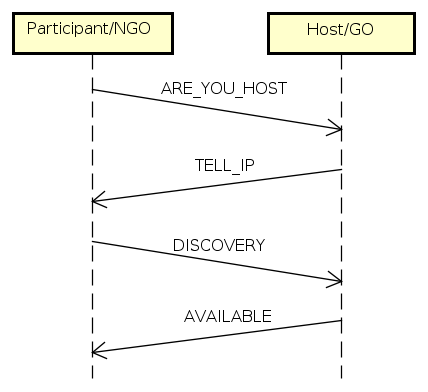
\includegraphics[width=0.30\textwidth]{SequenceDiagram1}
    \caption{Example of communication between a GO-host and an NGO-participant}
    \label{fig:seqDiagram1}
\end{figure}

\begin{figure}[h]
    \centering
    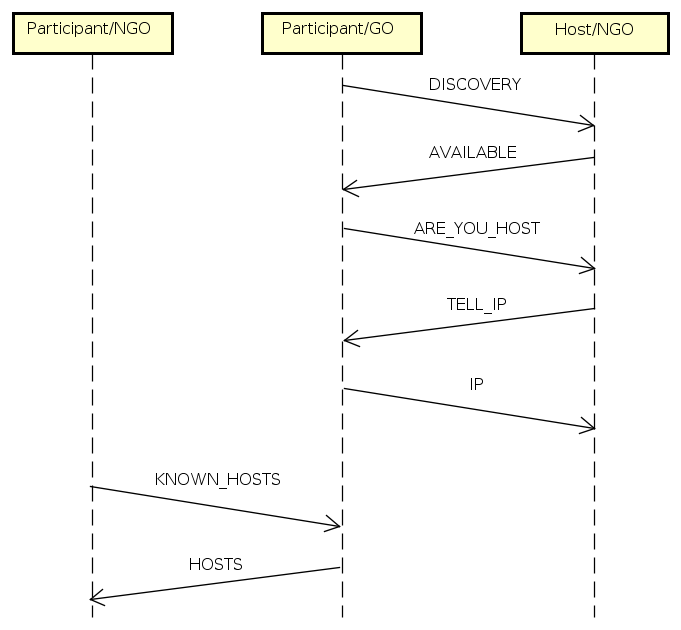
\includegraphics[width=0.30\textwidth]{SequenceDiagram2}
    \caption{Example of communication between an NGO-host, a GO-participant
     and an NGO-participant}
    \label{fig:seqDiagram2}
\end{figure}

Then the participant surely knows the IP of a host (if any) and it is able to
send a \texttt{DISCOVERY} message to the host. This message causes the host to
reply with an \texttt{AVAILABLE} message in which currently joined players are
listed. After this step, the participant can join the message by sending a
\texttt{JOIN} message to the host, receiving back an \texttt{AVAILABLE} message
in which she will be present as a confirmation. Finally, a player can cancel
her subscription by sending a \texttt{CANCEL} message and receiving back an
\texttt{AVAILABLE} message in which she will not be present anymore.

\begin{figure}[h]
    \centering
    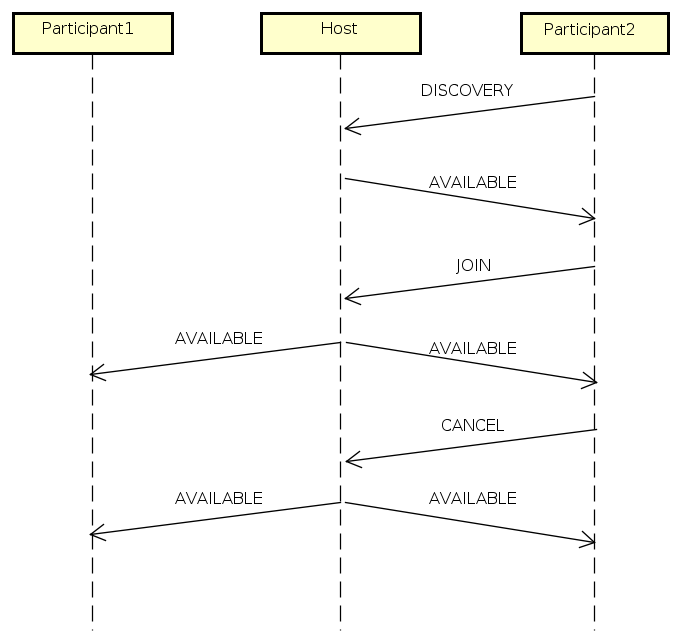
\includegraphics[width=0.30\textwidth]{SequenceDiagram3}
    \caption{Example of communication between a host and two participants,
     in which \emph{Participant1} has just joined the match and
     \emph{Participant2} has not}
    \label{fig:seqDiagram3}
\end{figure}

When a host player sees more than one participant in her match list, she can
decide to start a game, making her Multipong app send a \texttt{STARTING}
message to all of the game participants. Since this is a blocking operation
because it is better not to start the game until all the other players' games
started, the host has to wait for all the messages in its sending queue to be
sent before starting. If some player is unreachable for some reason
during the game starting, she will be excluded by the match as described in
the following subsection.



\subsection{Gameplay}

\begin{figure}[H]
    \centering
    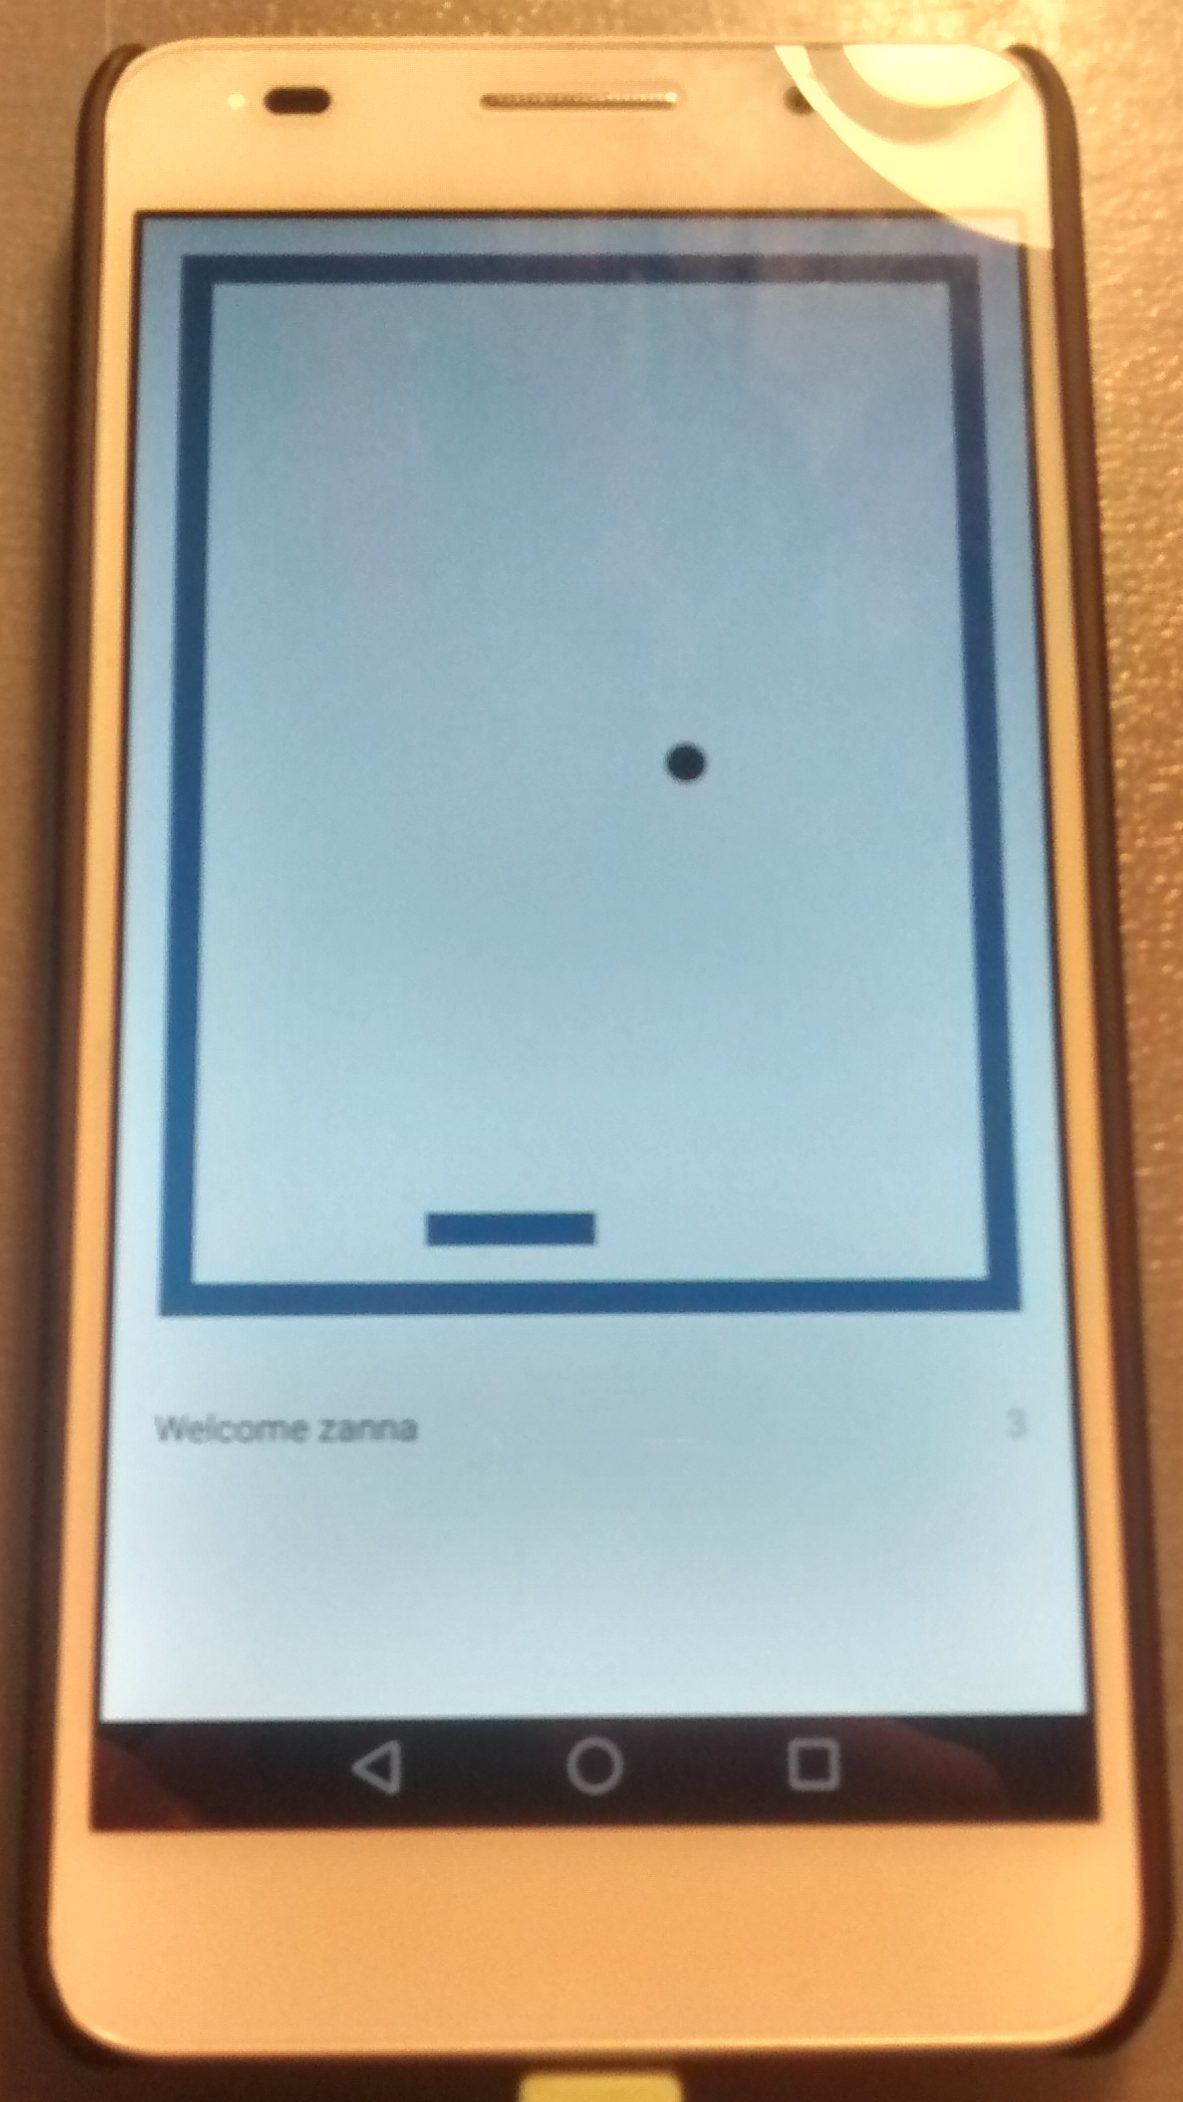
\includegraphics[height=0.23\textwidth]{singleplayer}
    \caption{Photo of a singleplayer match}
    \label{fig:singleplayer}
\end{figure}

\begin{figure}[H]
    \centering
    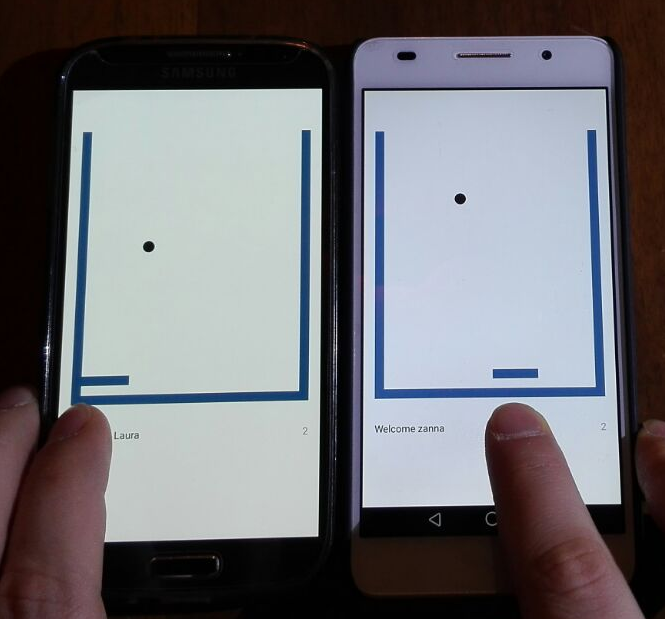
\includegraphics[width=0.23\textwidth]{multiplayer}
    \caption{Photo of a multiplayer match - Thanks to the prediction of ball 
     position, we could make appear the ball in the next devices before it 
     disappear from the first one, in order to have a more rapid and enjoyable 
     game experience}
    \label{fig:multiplayer}
\end{figure}

As anticipated, during the gameplay phase we changed direction regarding the
way we exchange data among peers. In fact, game information messages have to
be delivered very quickly and therefore TCP could not be the best choice for
fast delivery of data. We decided to make peers communicate to each other by
means of an application-level acked UDP transmission: after sending an UDP
packet, a peer waits for a short ACK packet to come back within a short time
frame; if it does not, the peer retries the transmission up to four times in
total.

In this phase of the game we want to have both consistency and low latency, so
that the game can be enjoyable. In order to do so, we designed a two layered
architecture, with one layer that is concerned with coordinating the peers and
the other one that deals with the multiplayer game logic on top of the
coordination layer.

The multiplayer game logic layer has to manage the local state of the game and
part of the global state. Also, when the player hits the ball with the paddle,
it also have to compute the ball exit point from the screen as send this
information to the GO as soon as it is available, so that it can spread this
message to all the active participants of the game. We chose to compute and
send the ball exit position in advance in order to reduce the network latency
perceived by the player.

Just here above we said that a player sends the game information to the GO:
in fact, this entity serves as a global coordinator of the game. We made this
decision so that a reduced amount of traffic has to flow through the network
if only the GO has to care about whether the currently active player is still
alive and reachable. Also, the GO is the main entity in the P2P group and this
makes it a natural choice for such a role like the coordinator.

Clearly, the GO represents a single point of failure during the game phase, but
we want to point out that a network failure such a crash of the coordinator
would make the whole ad-hoc network collapse. Moreover, recreating a P2P
network is an operation that, at the moment, is quite difficult to carry out
in a short amount of time (and unfortunately things go even worse when done
programmatically). Therefore, we thought that the game of an NGO should end if
it is unable to reach the GO, because restoring the game with the other active
players would be way worse than starting a new one from scratch.

While GO failures are fatal for the game, it copes better with NGOs failures:
in fact, if an NGO happens to look inactive for the GO, it is removed from the
game after the GO asked a few times if it is alive or not without getting any
response. In that case, the game continues with the GO telling the other
players that a certain peer is not active anymore.

A game always starts from the host device and the queue of players is decided
before the beginning of the match. Even if an NGO failure happens, the order of
the players' queue does not change but the player that is experiencing
networking problems is removed from the queue.
This strategy is not the only one possible.
In fact we could vary the order of the queue each turn, but we decided
not to follow this path for better testability and also because it would not
have been relevant for our analysis.

\section{Experimental evaluation}

In this section, we evaluate through different tests some interesting metrics
related to network activity. We used the following smartphones: 3 Samsung S5,
1 Samsung S3, 1 LG Nexus 5, 1 LG Nexus 5X, 1 LG Leon, 1 LG Spirit, 1 HTC Desire
S, 1 Honor 6, 1 Motorola Moto G 2013, 1 Motorola Moto X+1 2014, 1 Huawei P8
Lite.

\subsection{TCP and UDP packet RTT and payload}

We use TCP for message exchange during game formation phase, thus an interesting metric lies in application packet's RTT and payload.
 
To measure the RTT we decided to send a test-packet to a host which send it
back to the sender, then we obtain time delta between message start and
delivery. This should be an appropriate approximation of the RTT. This method
is affected by a little error due to network state variability and
interference, so we decided to take several measures and then average them.
Also, there is an overhead due to the time spent by the operating system to
manage the communication among devices.

For the TCP payload evaluation, we generated some logs in the application to get the exact size of each type of message. Messages always carry the same data structure and length, so in this case it is not necessary to calculate a mean value.

As for the TCP packets, we are interested in UDP RTT and payload statistics, so we measured them with the same approaches.

\subsection{\wifi{} traffic}

A more interesting evaluation is about general traffic over \wifi. The application was designed to minimize message exchange among peers, so we were interested in knowing how much traffic our application generates. To determine that, we decided to use, among the alternatives available on the market, an external monitoring application called \textit{3G Watchdog} (3GW from now on) [add reference]. This application is intended to monitor long-time traffic such as mobile connection over month/week, but it also keeps track of the time the application has run, so we were able to calculate both traffic and mean bandwidth allocation.

Multipong, anyway, generates different amounts of traffic in the various
phases. In fact, during the game creation the traffic is way more variable than
in the gameplay phase, mainly due to unstable number of peers and \wifi{}
interferences.

So, we decided to take measures of several game matches and then average them to get a minimal variation, applying the following workflow for each new match:

\begin{enumerate} % TODO: was it better an itemize?
  \item Start 3GW and reset its data counters
  \item Start a new game and play, possibly trying to variate match duration
  \item Annotate game transferred data and game duration
\end{enumerate}

This approach made us able to minimize the variability due to interferences, but the number of peers was still affecting considerably these measurements. So, we decided to group them by number of peers; more precisely, we chose to make 2-, 3- and 4-player matches. The comparison among these groups reveals the influence of the pairing phase to the traffic.

\subsection{Battery Consumption}

Usually, apps which do a massive use of \wifi{} are also highly energy-consuming. One of our minor purposes was to optimize the battery-life of the devices running our application, so we decided to track power consumption over the game. We identified a nice tool for energy monitoring in \textit{PowerTutor} (PT hereafter), a free application available on Google Play Store, widely used by the Android Development community. Clearly, this kind of applications are not able to do physical measures of the energy consumption, they just estimate it through a mathematical model created over results retrieved from some Android devices\footnote{in this case HTC G1, G2, G3 and Nexus One, though we were not able to run our application over these phones}.

This approach is however considered quite reliable in those cases where energy monitoring is not the core of the observation. Nevertheless, because of our communication minimization approach, we decided to compare energy consumption in multiplayer mode against the single-player mode, and because of different traffic on GOs and NGOs we also decided to consider separately these two scenarios.

\section{Results}

\subsection{Messages size}

Hereafter we list the messages peers exchange in Multipong and their
size\footnote{the size shown in the table has to be intended as ``greater or
equal than''}:

\begin{table}[H]
  \centering
  \begin{tabular}{l|c c}
  & \textbf{\textit{Message}} & \textbf{\textit{Size [B]}}  \tabularnewline
            \hline
            \multirow{5}{*}{TCP} & \multicolumn{1}{c}{\texttt{ARE\_YOU\_HOST}} & \multicolumn{1}{c}{60} \\\cline{2-3}
                                 & \multicolumn{1}{c}{\texttt{AVAILABLE}} & \multicolumn{1}{c}{100} \\\cline{2-3}
                                 & \multicolumn{1}{c}{\texttt{CANCEL}} & \multicolumn{1}{c}{56} \\\cline{2-3}
                                 & \multicolumn{1}{c}{\texttt{DISCOVERY}} & \multicolumn{1}{c}{82} \\\cline{2-3}
                                 & \multicolumn{1}{c}{\texttt{JOIN}} & \multicolumn{1}{c}{54} \\\hline
            \multirow{3}{*}{UDP} & \multicolumn{1}{c}{\texttt{KNOWN\_HOSTS}} & \multicolumn{1}{c}{90} \\\cline{2-3}
                                 & \multicolumn{1}{c}{\texttt{STARTING}} & \multicolumn{1}{c}{187} \\\cline{2-3}
                                 & \multicolumn{1}{c}{\texttt{TELL\_IP}} & \multicolumn{1}{c}{57} \\\hline
        \end{tabular}
  \caption{Messages size}
  \label{tab:sizes}
\end{table}

\subsection{Energy and traffic}

The average power consumption and Wi-Fi direct traffic can be seen in Figure
\ref{fig:comparison}.

\begin{figure}[H]
  \centering
  \begin{tabular}{@{}c@{}c}
      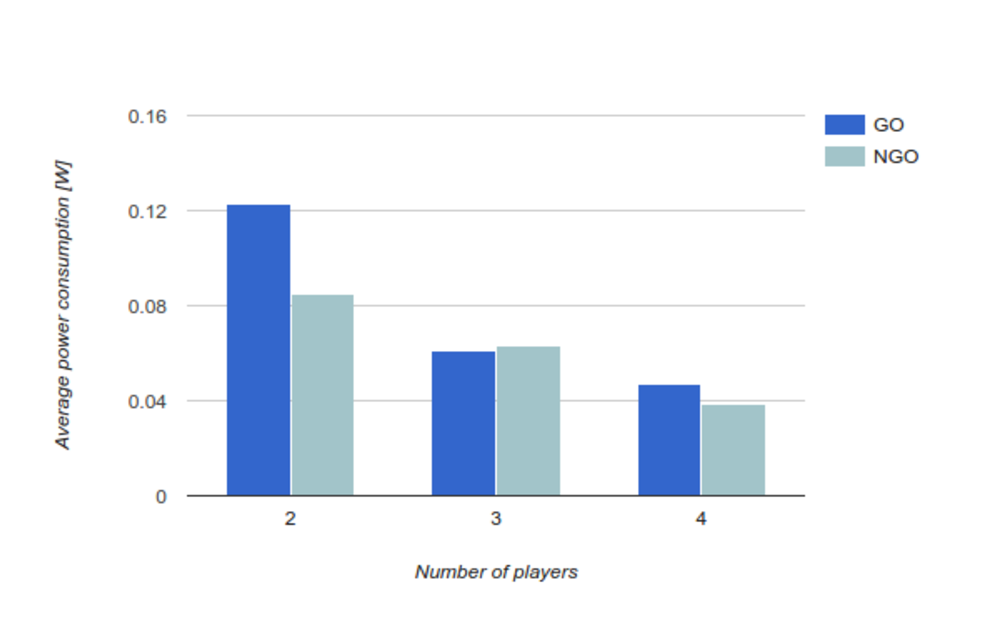
\includegraphics[width=.5\columnwidth]{img/energy.eps}
      \label{fig:energy}
    &
    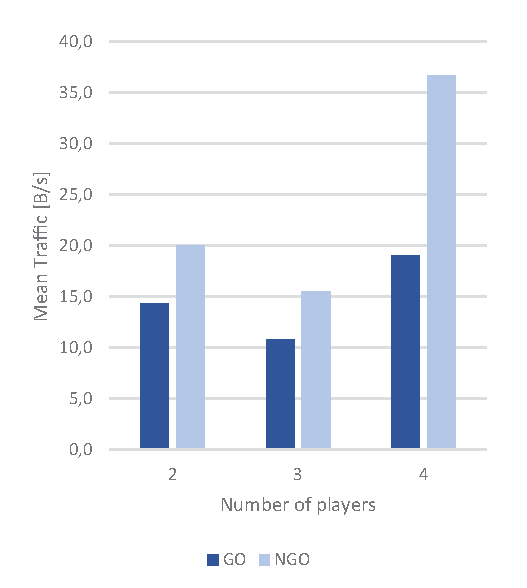
\includegraphics[width=.5\columnwidth]{img/traffic.eps}
    \label{fig:traffic}
  \end{tabular}
  \caption{GO/NGO comparison for energy and traffic}\label{fig:comparison}
\end{figure}

We notice that we have a lot of variability in power consumption because of
many factors, among which (1) the network instability, (2) user interaction
(the more the user touches the screen, the more power is consumed) and (3)
PowerTutor is not a truly reliable instrument to measure battery consumption 
because we used different devices from the ones used to create
PowerTutor's mathematical model. Hence, we can not say too much about how power
consumption varies depending on the number of players. Still, we noticed that
Multipong is quite light compared to other multimedia applications in terms of
battery consumption.

On the other hand, the figures about Wi-Fi traffic reveal that the number of
packets exchanged among the devices increases with the number of players. Often
the GO incurs less traffic than an NGO: we think this is because of iterated
attempts made by the NGOs to concurrently communicate to the GO, whereas
there is far less traffic (on average) when the GO has to send packets. In
particular, we are referring to both the liveness checks and the protocol
employed in the gameplay phase, since the GO has to spread information to all
the participants, which are diligently waiting for it.

\subsection{TCP and UDP comparison}

In Figure \ref{fig:TCP-UDP}, we can see the difference between the mean RTTs of
TCP and acked UDP transmissions.

\begin{figure}[H]
  \centering
  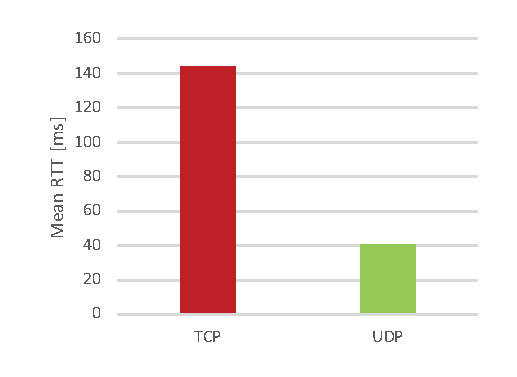
\includegraphics[width=.8\columnwidth]{img/UDPvsTCP-RTT.eps}
  \caption{TCP vs. UDP}
  \label{fig:TCP-UDP}
\end{figure}

As it can be easily seen, acked UDP is very efficient compared to TCP and
therefore we can acknowledge that acked UDP is the most suitable choice (between
these two) in the gameplay phase, whilst TCP is fit for the game formation
phase, when we do not need low latency but more reliable packet delivery.

\section{Conclusion}
%%*************************************************************************
In this paper we have presented issues and possibile solution that we 
encounter developing a simple multiplayer game based on Wi-Fi Direct 
technology. The main problem that we met is that the connection between 
different peers with Wi-Fi direct is really cumbersome. This must be done 
using Android settings and very often it takes too much time. 

Another problem is manage the unreachability of the GO in a Wi-Fi Direct
network. At the current state of art the best solution, for us, is what we 
implemented, that is interrupt the current match, because of the 
impossibility to reconstruct the network in a short time and automatically.

A further issues that we noticed is that the Wi-Fi Direct connection 
between two different devices could be easily disturbed trying to connect 
to one of the two devices with another one. Most of the times, in that case
the only thing to do is to cancel the request of connection and restart the 
formation of the network.

On the other hand, if the network is created correctly and there are not 
some other devices that try to join the network, we find out that the game 
is enjoyable and the Wi-Fi Direct could be a quite good solution for 
multiplayer mobile games.

% An example of a floating figure using the graphicx package.
% Note that \label must occur AFTER (or within) \caption.
% For figures, \caption should occur after the \includegraphics.
% Note that IEEEtran v1.7 and later has special internal code that
% is designed to preserve the operation of \label within \caption
% even when the captionsoff option is in effect. However, because
% of issues like this, it may be the safest practice to put all your
% \label just after \caption rather than within \caption{}.
%
% Reminder: the "draftcls" or "draftclsnofoot", not "draft", class
% option should be used if it is desired that the figures are to be
% displayed while in draft mode.
%
%\begin{figure}[!t]
%\centering
%\includegraphics[width=2.5in]{myfigure}
% where an .eps filename suffix will be assumed under latex, 
% and a .pdf suffix will be assumed for pdflatex; or what has been declared
% via \DeclareGraphicsExtensions.
%\caption{Simulation results for the network.}
%\label{fig_sim}
%\end{figure}

% Note that the IEEE typically puts floats only at the top, even when this
% results in a large percentage of a column being occupied by floats.


% An example of a double column floating figure using two subfigures.
% (The subfig.sty package must be loaded for this to work.)
% The subfigure \label commands are set within each subfloat command,
% and the \label for the overall figure must come after \caption.
% \hfil is used as a separator to get equal spacing.
% Watch out that the combined width of all the subfigures on a 
% line do not exceed the text width or a line break will occur.
%
%\begin{figure*}[!t]
%\centering
%\subfloat[Case I]{\includegraphics[width=2.5in]{box}%
%\label{fig_first_case}}
%\hfil
%\subfloat[Case II]{\includegraphics[width=2.5in]{box}%
%\label{fig_second_case}}
%\caption{Simulation results for the network.}
%\label{fig_sim}
%\end{figure*}
%
% Note that often IEEE papers with subfigures do not employ subfigure
% captions (using the optional argument to \subfloat[]), but instead will
% reference/describe all of them (a), (b), etc., within the main caption.
% Be aware that for subfig.sty to generate the (a), (b), etc., subfigure
% labels, the optional argument to \subfloat must be present. If a
% subcaption is not desired, just leave its contents blank,
% e.g., \subfloat[].


% An example of a floating table. Note that, for IEEE style tables, the
% \caption command should come BEFORE the table and, given that table
% captions serve much like titles, are usually capitalized except for words
% such as a, an, and, as, at, but, by, for, in, nor, of, on, or, the, to
% and up, which are usually not capitalized unless they are the first or
% last word of the caption. Table text will default to \footnotesize as
% the IEEE normally uses this smaller font for tables.
% The \label must come after \caption as always.
%
%\begin{table}[!t]
%% increase table row spacing, adjust to taste
%\renewcommand{\arraystretch}{1.3}
% if using array.sty, it might be a good idea to tweak the value of
% \extrarowheight as needed to properly center the text within the cells
%\caption{An Example of a Table}
%\label{table_example}
%\centering
%% Some packages, such as MDW tools, offer better commands for making tables
%% than the plain LaTeX2e tabular which is used here.
%\begin{tabular}{|c||c|}
%\hline
%One & Two\\
%\hline
%Three & Four\\
%\hline
%\end{tabular}
%\end{table}


% Note that the IEEE does not put floats in the very first column
% - or typically anywhere on the first page for that matter. Also,
% in-text middle ("here") positioning is typically not used, but it
% is allowed and encouraged for Computer Society conferences (but
% not Computer Society journals). Most IEEE journals/conferences use
% top floats exclusively. 
% Note that, LaTeX2e, unlike IEEE journals/conferences, places
% footnotes above bottom floats. This can be corrected via the
% \fnbelowfloat command of the stfloats package.








% conference papers do not normally have an appendix


% use section* for acknowledgment
\section*{Acknowledgment}


The authors would like to thank...





% trigger a \newpage just before the given reference
% number - used to balance the columns on the last page
% adjust value as needed - may need to be readjusted if
% the document is modified later
%\IEEEtriggeratref{8}
% The "triggered" command can be changed if desired:
%\IEEEtriggercmd{\enlargethispage{-5in}}

% references section

% can use a bibliography generated by BibTeX as a .bbl file
% BibTeX documentation can be easily obtained at:
% http://mirror.ctan.org/biblio/bibtex/contrib/doc/
% The IEEEtran BibTeX style support page is at:
% http://www.michaelshell.org/tex/ieeetran/bibtex/
%\bibliographystyle{IEEEtran}
% argument is your BibTeX string definitions and bibliography database(s)
%\bibliography{IEEEabrv,../bib/paper}
%
% <OR> manually copy in the resultant .bbl file
% set second argument of \begin to the number of references
% (used to reserve space for the reference number labels box)
\begin{thebibliography}{1}

%%%     bib separator     %%%
\bibitem{bib:newzoo2}
Newzoo Games,
\emph{The Global Games Market Reaches \$99.6 Billion in 2016,
Mobile Generating 37\%}. April 2016.
%%%     bib separator     %%%
\bibitem{bib:newzoo}
Newzoo Games, \emph{Free 2016 Global Games Market Report: An overview of
trends \& insights}. June 2016.
%%%     bib separator     %%%
\bibitem{bib:moeller-qoe}
Möller, S., Schmidt, S. and Beyer, J.,
\emph{Gaming Taxonomy: an Overview of Concepts And Evaluation Methods for
Computer Gaming QoE}.
In Quality of Multimedia Experience (QoMEX), 2013 Fifth International Workshop
on (pp. 236-241). IEEE.
%%%     bib separator     %%%
\bibitem{bib:wifiP2pspec}
Wi-Fi Alliance\textsuperscript{\textregistered},
\emph{Wi-Fi Peer-to-Peer (P2P) Technical Specification v1.7}.
July 2016
%%%     bib separator     %%%
\bibitem{bib:ppav-casual}
Paavilainen, J., Annakaisa K., Jussi K., Frans M., Hannamari S., and Johannes
N.,
\emph{GameSpace: Methods and Evaluation for Casual Mobile Multiplayer Games}.
2009
%%%     bib separator     %%%
\bibitem{bib:li-k-social-casual}
Li, K., and Counts, S.,
\emph{Exploring social interactions and attributes of casual multiplayer
mobile gaming}.
In Proceedings of the 4th international conference on mobile technology,
applications, and systems and the 1st international symposium on Computer
human interaction in mobile technology, pp. 696-703.
ACM, 2007.
%%%     bib separator     %%%
\bibitem{bib:mob-health-casual}
Grimes, A., Kantroo, V. and Grinter, R.E.,
\emph{Let's play!: mobile health games for adults}.
In Proceedings of the 12th ACM international conference on Ubiquitous
computing (pp. 241-250).
ACM, September 2010
%%%     bib separator     %%%
\bibitem{bib:android-wifidirect-limits}
Stefano Cappa,
\emph{Analisi dei limiti dell'implementazione di Wi-Fi Direct in Android per
reti opportunistiche}.
\url{http://hdl.handle.net/10589/107204}.
April 2015
%%%     bib separator     %%%
\bibitem{bib:interactive-mobile-gaming}
Claudio E. Palazzi,
\emph{Interactive Mobile Gaming over Heterogeneous Networks}.
In Proc. of the 5th IEEE/ITI International Conference on Information and
Communications Technology (ICICT 2007), Cairo, Egypt,
December 2007.
%%%     bib separator     %%%
\bibitem{bib:mobile-input-devices}
Chu, K. and Wong, C.Y.,
\emph{Mobile input devices for gaming experience}.
In User Science and Engineering (i-USEr), 2011 International Conference on
(pp. 83-88). IEEE.
November 2011

Chu Kimberly, Chui  Yin Wong,
\emph{Mobile input devices for gaming experience}, 
November 2011
%%%     bib separator     %%%
\bibitem{bib:can-mobile-gaming-be-improved}
Tobias Fritsch, Hartmut Ritter, Jochen Schiller
\emph{CAN mobile gaming be improved?}
%%%     bib separator     %%%
\bibitem{bib:study-mobile-phone-sector}
Tobias Fritsch, Hartmut Ritter, Jochen Schiller
\emph{User Case Study and Network Evolution in the Mobile Phone Sector
 (A study on current mobile phone applications)}
\end{thebibliography}


% that's all folks
\end{document}


